\chapter{Results}

\section{Abstract model for DAO units}

It is better to draw easier-to-understand pictures. Explanation: \ldots

In following examples this model will be set up to act similarly like NP: $\exists y \; R(x,y)$. Although existence is not sure it is very likely. Predicate $R$ will be enumerable in polynomial time for $x \in L$. In this context, {\em enumerable in polynomial time} will mean number of bindings, not number of biosteps. This can be assumed due to Turing universality of this model in $O(1)$ biosteps, thus biostep complexity is not restrictive and will be required to be $O(1)$. On the other hand the binding complexity will be very important, we will be interested even in constants. This is because the less binding complexity, the less probability of error.

Define (slightly more correctly) binding complexity of this model as the number of bindings. Only the biggest term will be considered but even with constant.

% ňák líp, taky by stálo za to zmínit, že víc biostepů nevede k větší třídě vyčíslitelných funkcí (taky když už tady mam Turing universal že ...)
% diskutovat pravděpodobnost objevení vs. neobjevení $y$ !!! dát odkaz do footnote

\section{Graph 3-coloring}

Remind original Knuth's algorithm at \url{http://www.iti.fh-flensburg.de/lang/algorithmen/sortieren/networks/oetsen.htm}! And prove that everything goes fine!

First idea: Generate all bonds with colored atoms and check the entire system (haha, complexity like $O(n^4)$ because $|E| \in O(n^2) $). Second solution: Generate a reverse-order sequence of vertices and let it order in the correct order. All pairs should meet each other, the problem to solve is whether all pairs really meet each other. After that check that the area is full like Winfree -- from one side to the other. Improvement: the check can be triggered from both sides simultaneously.

The first idea was like $O(n^4)$, the second one is already $O(n^2)$, the binding complexity is $1\nicefrac{1}{2}\;n^2$. The improvement decreases it to $1\nicefrac{1}{4}\;n^2$.

\begin{figure}[h]
\begin{center}
	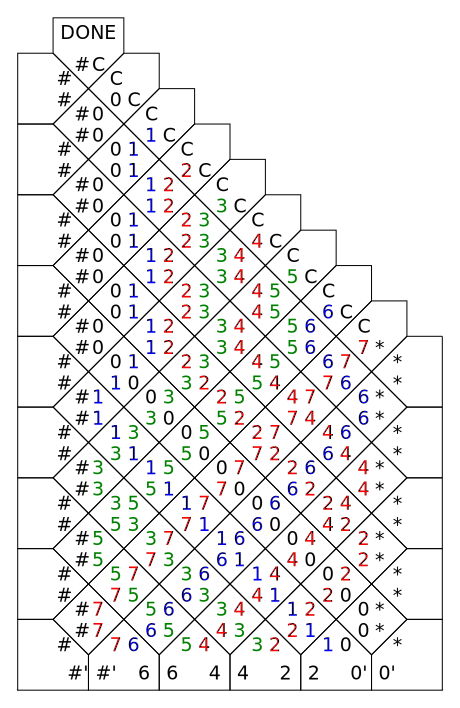
\includegraphics[scale=0.85]{./figures/3-color/3-color.pdf}
	\caption{3-color computation}
\end{center}
\end{figure}

\section{Graph isomorphism}

Graph isomorphism problem clearly belongs to NP but it does not seem to be NP-hard\footnote{Clearly, if P = NP it would even belong to P.} \cite{borec_z_wiki}. Thus it seems that it is neither P nor NP-complete. From this reason it seems to belong to a special class and thus I will describe a DNA system which solves this problem. % and if it were NP-hard there would collapse some complexity classes, see wiki

Surprisingly it is very similar to 3-coloring if we consider $n$ colors instead. Each color will be assigned to concrete vertex. But there are slight differences, one has to check whether:
\begin{enumerate}
	\item edges and non-edges are preserved,
	\item every ``color'' was used exactly once.
\end{enumerate}
In the first step the difference is that one checks coincidence of more cases. In the second step a similar check procedure is to be performed.

% zjistit jesli ověřuje že se použijou všechny..? že se nepoužije nic dvakrát? jasně! až dojedu srovnání podle primárního klíče (který zaručí že se každý dva potkaj) rozjedu druhý který srovná sekundární klíč a ten následně zkontroluju jako Winfree že tam je všechno právě jednou! :) .. místo na trik

\begin{figure}[h]
\begin{center}
	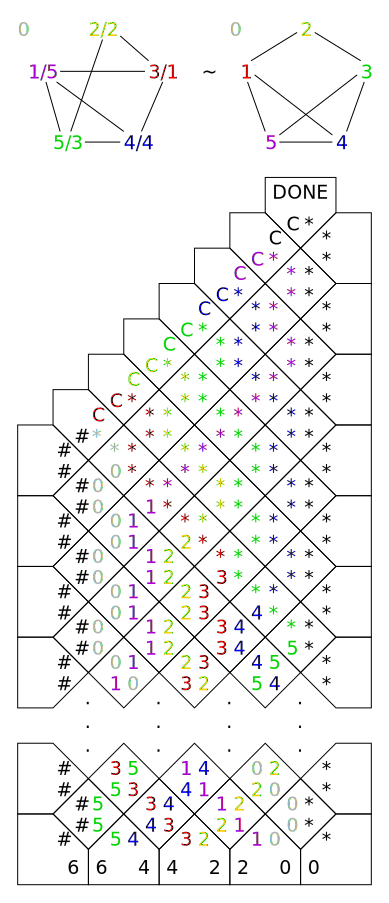
\includegraphics[scale=0.85]{./figures/isomorphism/isomorphism.pdf}
	\caption{Graph isomorphism}
\end{center}
\end{figure}
